\chapter{Aspectos Conceituais}
    
    \section{Ambiente de desenvolvimento}
    
    O ambiente de desenvolvimento de um projeto de desenvolvimento de software é o termo usado para todos os itens de que o projeto precisa para desenvolver e implantar o sistema, como, por exemplo, ferramentas, diretrizes, processo, \textit{templates} e infra-estrutura.\cite{ambientedev}
    
    Geralmente temos alguns ambientes de de software bem comuns como Produção, Homologação e Desenvolvimento. Cada um desses ambientes possui suas características próprias e requisitos de funcionamento e ferramental.
    
    Em especial o ambiente de desenvolvimento incluem as ferramentas utilizadas pelo desenvolvedor para escrever, executar e testar sua aplicação, nesse contexto temos editores de texto, ferramentas de linha de comando, executores de teste, plataformas de contêineres locais para execução de serviços, entre outros.
    
    \section{Desenvolvimento em tempo real} %% TODO
    
    Quando falamos de "tempo real" esperamos que o tempo entre ação e \textit{feedback} seja curto o suficiente para atender os requisitos de uma determinada aplicação. No caso de desenvolvimento em tempo real, queremos que o tempo de iteração no processo de escrita de código e validação deste, seja curto o suficiente para não prejudicar o fluxo de desenvolvimento do desenvolvedor, geralmente estamos falando de algo na casa de segundos até poucos minutos.
    
    Esse tempo pode ser por exemplo, o intervalo de tempo levado para execução de testes unitários ou de integração que são usados pelo desenvolvedor. Aqui não se incluem processos que são executados em pipelines automatizadas ou sistemas de CI/CD, somente as ferramentas utilizadas pelo desenvolvedor no dia a dia.
    
    \section{Contêineres} %% TODO: Paps 
	    \subsection{Breve história da tecnologia}
	    A história dos Contêineres começa em 1979 no Unix L7. Nele foi introduzido a chamada de sistema (\textit{system call}) \textit{chroot} capaz de mudar o diretório raiz de um processo e de seus processos filhos para um novo local no sistema de arquivos. Este avanço foi o início do conceito de isolamento de processos, pois limitava o acesso de cada processo ao sistema de arquivos. 

	    Em 2000, surgiu o FreeBSD Jail, que permitia a administradores particionar um sistema FreeBSD em vários sistemas menores isolados e independentes, chamados de “\textit{jails}”. O sistema é similar ao \textit{chroot}, mas incluiu recursos de isolamento adicionais em diversos aspectos do sistema operacional, como por exemplo a atribuição de um endereço de IP diferente para cada \textit{jail}. \cite{abriefhistoryofcontainers}

	    Em 2001, foi lançado o Linux VServer que, assim como o FreeBSD Jail, também é um mecanismo de \textit{jail} que pode particionar recursos (sistema de arquivos, endereços de rede, memória) em um sistema computacional. Isso é realizado por meio de níveis de isolamento do \textit{kernel}. Cada partição é chamada \textit{security context} e o sistema virtualizado dentro dele é chamado de \textit{virtual private server}. \cite{linuxvserver}

    	Em 2004, foi lançado o Solaris Zones para sistemas x86 e SPARC. Cada \textit{zone} age como um servidor virtual completamente isolado dentro de uma única instância. Existem dois tipos de \textit{zones}: zonas globais (\textit{Global Zones}) e não-globais (\textit{Non-Global Zones}). A zona global é o ambiente de SO tradicional e é a área onde o SO Solaris está instalado. Todas as operações do sistema, como instalações, inicializações e desligamentos são feitas na zona global. As zonas não-globais, comumente chamadas somente de zonas, tem seus recurso e limites definidos pela zona global a que pertencem  \cite{introductiontosolariszone}

    	Em 2005 a empresa Virtuozzo lançou o OpenVZ, que utiliza o \textit{kernel} do Linux para fornecer virtualização, isolamento, gerenciamento de recursos e \textit{checkpointing}. Cada contêiner OpenVZ possui um sistema de arquivos isolado, usuários e grupos de usuários, uma árvore de processos, rede, dispositivos e comunicação entre processos. Uma desvantagem da solução é que seu funcionamento depende da aplicação de um \textit{patch} no \textit{kernel} do Linux. \cite{openvz}

    	Em 2006 engenheiros da Google desenvolveram o Process Containers, projetado para limitar, contabilizar e isolar o uso de recursos computacionais (CPU, memória, I/O do disco, rede) de uma coleção de processos. Um ano depois o projeto foi renomeado para Control Groups (\textit{cgroups}) e foi adicionado ao \textit{kernel} do Linux na versão \textit{2.6.24}.

    	Em 2008 surgiu o LXC (LinuX Containers), que foi a primeira e mais completa implementação de um gerenciador de contêineres Linux. Foi implementado utilizando \textit{cgroups} e Linux \textit{namespaces} e funciona no \textit{kernel} do Linux sem a necessidade da aplicação de \textit{patches}.
	
    	Em 2011 a empresa CloudFoundry iniciou o projeto Warden, que utilizava LXC em suas primeiras implementações, porém depois foi substituído por soluções próprias da empresa. Warden roda em formato \textit{daemon} e pode isolar ambientes em qualquer sistema operacional. Além disso, provê uma API para o gerenciamento de \textit{cgroups}, \textit{namespaces}, ciclo de vida dos processos e dos contêineres em diversos \textit{hosts} através de um modelo cliente-servidor.

    	Finalmente, em 2013, surgiu o Docker. Neste momento contêineres cresceram muito em popularidade, juntamente com o Docker em si.
	    Assim como o Warden, o Docker utilizou LXC em seus primeiros estágios mas logo trocou por uma solução própria para gerenciamento de     contêineres: o \textit{libcontainer}.
	    O Docker se destacou de seus concorrentes por oferecer um ecossistema completo para o gerenciamento de contêineres, que será detalhado mais adiante.
	
	\subsection{Diferenças com Máquinas virtuais}
	
	A virtualização é a tecnologia que permite a criação de diferentes ambientes computacionais, chamados de virtuais por simular a interface que é esperada por um sistema operacional.
	
	Um dos principais componentes da arquitetura é o \textit{Hypervisor}. Ele gerencia a distribuição dos recursos computacionais na máquina física (armazenamento, processamento e memória) entre as várias máquinas virtuais, além de fornecer um isolamento entre elas. Ele é um componente que fica entre o \textit{hardware} e a máquina virtual e é necessário para o processo de virtualização.
	Entre os gerenciadores de máquinas virtuais mais populares no mercado, pode-se citar VMWare vSphere, VirtualBox, Xen, Hyper-V e KVM.

	No baixo nível, um contêiner é apenas um conjunto de processos que são isolados do resto do sistema. No caso do Docker, os contêineres compartilham o \textit{kernel} do sistema operacional hospedeiro e, frequentemente, os binários e bibliotecas também. Todos os componentes compartilhados são \textit{read-only}. Este compartilhamento de componentes reduzem a necessidade de se replicar código do sistema operacional, e isso significa que um único servidor pode executar múltiplos contêineres com uma única instalação do sistema operacional.

	Diferentemente, uma máquina virtual é constituída do espaço de usuário juntamente com o espaço do \textit{kernel} de um sistema operacional e o \textit{hardware} é virtualizado. Cada máquina virtual tem um sistema operacional e suas aplicações e elas compartilham entre si o \textit{hardware} do computador hospedeiro.

	Ambas as tecnologias provém ambientes isolados para execução de aplicações e podem ser utilizadas para empacotar e distribuir \textit{software}.

	Dado o menor número de camadas entre a aplicação e o \textit{hardware},  os contêineres tendem a ser mais leves e mais rápidos, tornando-os mais práticos para os ciclos de desenvolvimento e implantação de serviços. Comparativamente, o tempo de inicialização de uma máquina virtual é muito maior do que a de um contêiner equivalente, além de o espaço ocupado em disco ser uma ordem de magnitude maior. \cite{whatsthediffvmvscontainers}
	
	\begin{figure}[htb]
		\caption{\label{fig_circulo}Diferenças entre VMs e Contêiners}
		\begin{center}
    		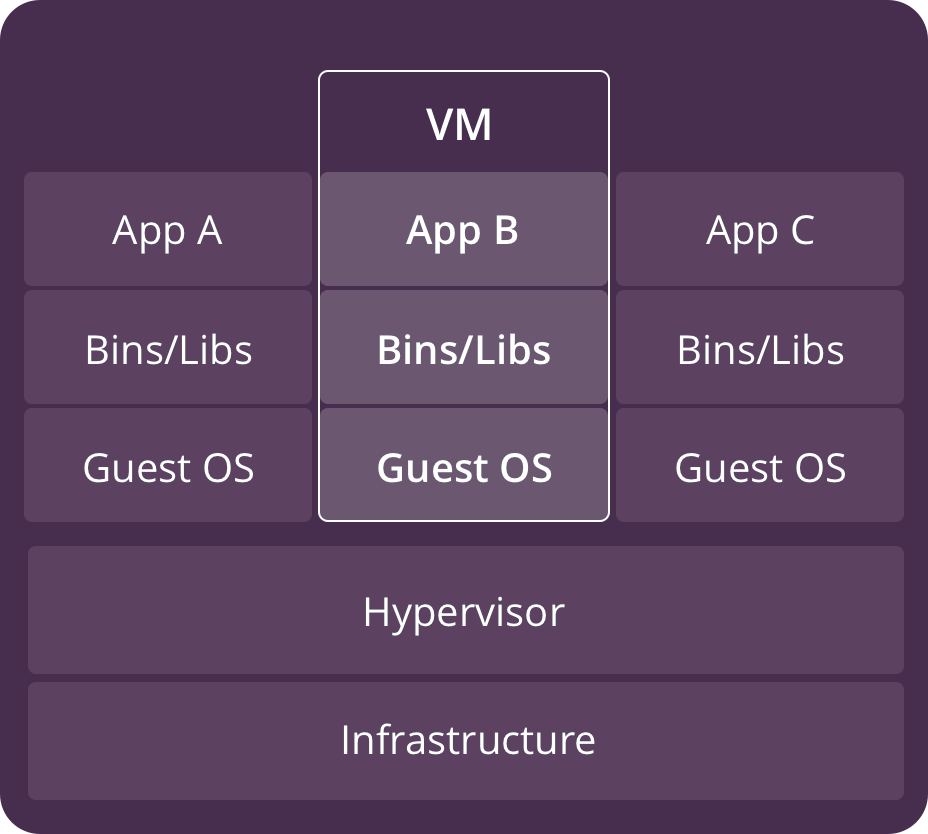
\includegraphics[scale=0.20]{pictures/vms.png}
    		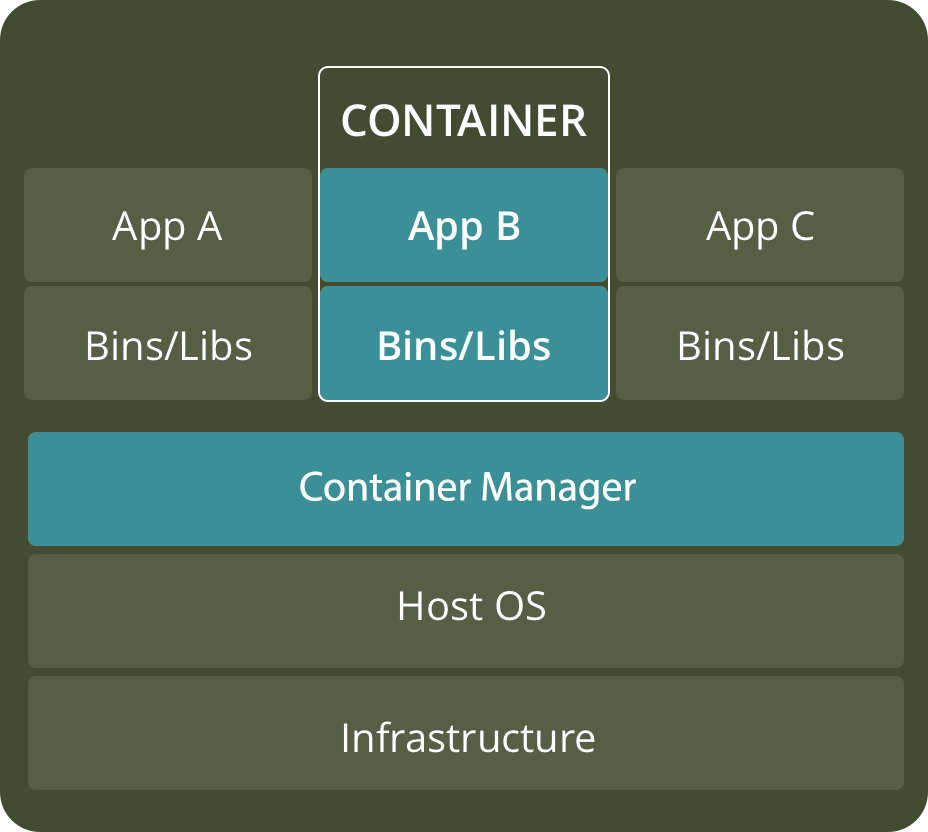
\includegraphics[scale=0.20]{pictures/containers.png}
		\end{center}
		\legend{Fonte: https://www.backblaze.com/blog/vm-vs-containers/}
	\end{figure}
	
	Ambos têm vantagens e desvantagens, e a decisão entre um outro varia dependendo dos casos de uso específicos, mas pode-se utilizar as seguintes regras como um ponto de partida:
	
	Máquinas virtuais são melhores para executar aplicações que necessitam de todos os recursos e funcionalidades do sistema operacional ou quando há uma variedade de sistemas operacionais para se gerenciar.
	
	Contêineres são uma escolha melhor quando a maior prioridade é maximizar o número de aplicações sendo executadas em um número mínimo de servidores.
	
	\section{Cloud Computing}
	Computação em Nuvem (do Inglês \textit{Cloud Computing}) é segundo a NIST \footnote{National Institute of Standards and Technology, https://www.nist.gov/} um modelo para prover um acesso de rede a um grupo compartilhado (\textit{shared pool}) de recursos computacionais (recursos como capacidade de rede, servidores, armazenamento, aplicações e serviços) de forma ubíqua, prática e sob demanda.

    Tal acesso deve ser rapidamente provisionado e lançado com o mínimo de gerenciamento e interação com o provedor de serviços por parte da aplicação.

    O modelo de computação em nuvem deve possuir algumas características básicas, que estão descritas na seção seguinte.

        \subsection{Características básicas de Cloud Computing}

            A NIST define 5 características essenciais do modelo de Cloud Computing:
            \begin{itemize}
            	\item Serviço sob demanda: Um consumidor pode provisionar unilateralmente capacidades computacionais, como tempo de servidor e armazenamento de rede, conforme for necessário, sem qualquer interação humana com o provedor de serviço;
            	
            	\item Agrupamento de recursos: Os recursos de computação do provedor são agrupados para atender a vários consumidores usando um modelo "multi inquilino", com diferentes recursos físicos e virtuais dinamicamente atribuídos e reatribuídos de acordo com a demanda do consumidor. Existe uma sensação de independência de localização pois o cliente geralmente não tem controle ou conhecimento sobre a localização exata dos recursos fornecidos, mas pode ser capaz de especificar a localização em um nível de abstração (por exemplo, país, estado ou datacenter). Exemplos de recursos incluem armazenamento, processamento, memória e largura de banda de rede.
            	
            	\item Amplo acesso à rede: Os recursos estão disponíveis na rede e são acessados por meio de mecanismos que promovam o uso por plataformas heterogêneas por clientes em diversos dispositivos (por exemplo, telefones celulares, tablets, laptops e estações de trabalho). Esta característica promove o conceito de computação ubíqua, isto é, em toda parte, onipresente.
            	
            	\item Elasticidade rápida: Os recursos podem ser provisionados e liberados elasticamente, em alguns casos automaticamente, proporcionando uma escalabilidade crescente ou descrescente conforme a demanda. Os recursos disponíveis normalmente aparentam ser ilimitados para o consumidor, podendo ser requisitidados em qualquer quantidade e a qualquer momento.
            	
            	\item Serviço mensurável: Os sistemas em nuvem controlam e otimizam automaticamente o uso de recursos, aproveitando-se de uma capacidade de medição em um nível de abstração apropriado ao tipo de serviço (por exemplo, armazenamento, processamento, largura de banda e contas de usuário ativas). O uso de recursos pode ser monitorado, controlado e reportado, gerando transparência tanto para o fornecedor e consumidor do serviço utilizado.
            \end{itemize}

        \subsection{Modelos para Cloud Computing}

        Este capítulo introduz brevemente os modelos de serviço de cloud computing que podem ser adotados por um provedor e os modelos de     \textit{deployment}, nas secções seguintes.

\subsection{Modelos de serviços}

A teoria por trás dos serviços de computação em nuvem abrange três elementos principais: software, plataforma e infraestrutura. Temos os seguintes modelos de serviço:

\begin{itemize}
  \item \textbf{SaaS, Software as a Service} ("Software como um serviço") 

  Neste modelo é oferecido ao consumidor o uso de aplicações de um provedor que rodam sobre uma infraestrutura em nuvem. Estas aplicações são acessíveis a partir de vários dispositivos clientes por meio de uma interface simples, como um navegador da web, ou uma interface de por meio de um programa (mobile ou desktop). 

  O consumidor não gerencia ou controla a infraestrutura de nuvem por trás da aplicação, incluindo rede, servidores, sistemas operacionais, armazenamento ou capacidade da aplicação individual. São disponibilizadas apenas configurações do aplicativo específicas para aquele usuário individual.

  Alguns exemplos de SaaS são serviços de \textit{webmail}, \textit{streaming} de vídeos, conversão de arquivos e trabalho colaborativo com arquivos. Este modelo não será mais detalhado neste trabalho.

  \item \textbf{PaaS, Platform as a Service} ("Plataforma como um serviço") 

  A capacidade fornecida ao consumidor é de implantar na nuvem aplicações criadas por meio de linguagens de programação, bibliotecas, serviços e ferramentas suportadas pelo provedor. Tais aplicações podem ser criadas pelo próprio consumidor, ou consumidas por este.

  Assim como no modelo de SaaS, o consumidor geralmente não gerencia ou têm controle sobre a infraestrutura de nuvem por trás, incluindo rede, servidores, sistemas operacionais, ou armazenamento. Porém o consumidor as tem controle sobre os aplicativos implantados e possivelmente sobre definições de configuração para o ambiente de hospedagem do aplicativo.

  Como exemplos de provedores no mercado temos \textit{IBM Bluemix}, \textit{Heroku}, e \textit{Windows Azure Cloud}.

  \item \textbf{IaaS, Infrastructure as a Service} ("Infraestrutura como um serviço") 

  A capacidade oferecida ao consumidor é provisionar processamento, armazenamento, redes e outros recursos fundamentais de computação onde o consumidor é capaz de implantar e executar software arbitrário, incluindo-se sistemas e aplicações. O consumidor não gerencia nem controla a infraestrutura de nuvem por trás, mas tem controle sobre sistemas operacionais, armazenamento e aplicativos implantados. Possivelmente possui também um controle limitado de componentes de rede (por exemplo, firewalls de host). Geralmente acompanha serviços de máquinas virtualizadas.

  Alguns exemplos de provedores no mercado são \textit{Amazon Web Services}, \textit{Microsoft Azure}, \textit{Google Cloud} e \textit{VMware Cloud on AWS}. 
\end{itemize}

	\section{Programação Funcional}
	
	Como o próprio nome diz, a programação funcional surge de funções matemáticas, mais especificamente do cálculo lambda. Programação funcional é um paradigma de programação assim como Orientado a Objeto ou Imperativo. As características mais marcantes desse paradigma são a presença de imutabilidade de dados e estados, funções serem tratadas como valores como quaisquer outros tipos (inteiros, strings, etc...), transparência referencial e separação de efeitos colaterais.
	As linguagens de programação podem ser puramente funcionais, ou parcialmente, isso é, contém elementos desse paradigma porém não se limitam a ele, ou fazem pequenos desvios em prol da usabilidade.
	
	\section{Microsserviços}
	
	Microsserviços é um termo usado para designar uma arquitetura de software distribuída que possui um certo conjunto de características, como por exemplo o deploy independente. É uma abordagem de desenvolvimento que que permite a criação de uma aplicação única através de um conjunto de pequenos serviços, de modo que cada um é responsável apenas por uma pequena parte do processo e durante sua execução eles se comunicam por meio de mecanismos leves, geralmente uma API e/ou mensageria (mas não se limitando a esses). Cada um dos serviços é focado em uma parte atômica da lógica de negócio e funcionam através de mecanismos de deploy independente e automatizado. Em contraste a esse tipo de arquitetura temos uma aplicação monolítica, que se caracteriza pela centralização da lógica e código em apenas um serviço de grande porte. \cite{microsservicos}
	
	\begin{figure}[htpb]
	    \caption{Microsserviços vs Monolitos}
	    \begin{center}
	        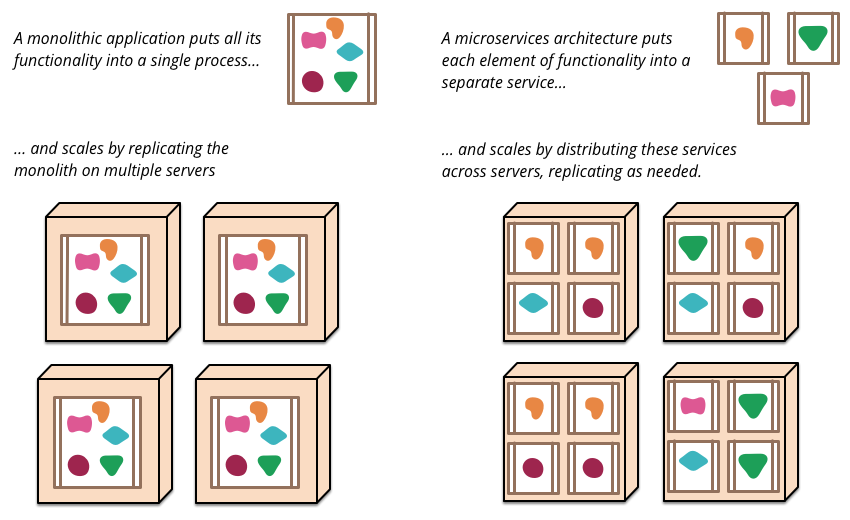
\includegraphics[scale=0.4]{pictures/sketch_microservices.png}
	    \end{center}
	    \label{fig:microsservicos_vs_monolito}
	    \legend{Fonte: https://martinfowler.com/articles/microservices/images/sketch.png}
	\end{figure}

    A arquitetura de microsserviços tem diversas vantagens em relação a monolítica, como por exemplo a divisão da lógica de negócio em pequenos serviços torna esses mais fáceis de compreender em relação a uma grande aplicação única. Esse modelo também torna mais simples a adoção de novas tecnologias sem a necessidade de intervir em serviços já existentes, isso acaba também por facilitar o desenvolvimento em equipe, dando mais independência para times entenderem e realizarem modificações em seus serviços, o que por fim contribui para o crescimento da empresa e sua escalabilidade.\cite{microservices-intro}
    
    Microsserviços também são uma opção altamente escalável e permitem que cada serviço seja dimensionando dinamicamente e individualmente em relação aos outros, o que significa que em arquiteturas de maior porte permite uma economia de recursos e melhor dimensionamento de capacidade dos serviços.
    
    Por outro lado, microsserviços também tem seu lado negativo, possuindo algumas desvantagens em relação ao modelo monolítico. Entre elas o sistema altamente distribuído exige que se tenha um alto nível de automação da infra-estrutura para que eles possam ser utilizados de forma fácil, como por exemplo o uso de algum PaaS. Gerenciamento de dados distribuídos, problemas de consistência eventual e lógica distribuída também se apresentam como desafios desse modelo de arquitetura.

	\section{Distributed Tracing}
	
	Distributed Tracing, ou Rastreamento Distribuído, é uma técnica utilizada em sistemas distribuídos para conseguir acompanhar algum fluxo que acaba por interagir com diversos serviços. Muito utilizado para ajudar desenvolvedor em sessões de depuração afim de entender qual caminho de código está sendo executado e com quais parâmetros em um sistema complexo e distribuído. Geralmente esse sistema se compõe de um broker central para onde as métricas e dados de tracing são enviados pelos serviços, e um conjunto de código que roda em todos os serviços, responsável por realizar a amostragem e enviar esses dados para o broker principal. Enquanto os brokers esperam receber mensagens representando eventos de entrada ou saída dos serviços através de um processo coletor, as bibliotecas se encarregam de enviar essa menagem e também propagar informações de rastreabilidade para as próximas interações com outros serviços. Podemos ver um digrama exemplificando a arquitetura de um Distributed Tracing nas figuras \ref{fig_tracing_concept} e \ref{fig_tracing_components}
	
	\begin{figure}[htb]
		\caption{\label{fig_tracing_concept}Anatomia de um Distributed Tracing}
		\begin{center}
		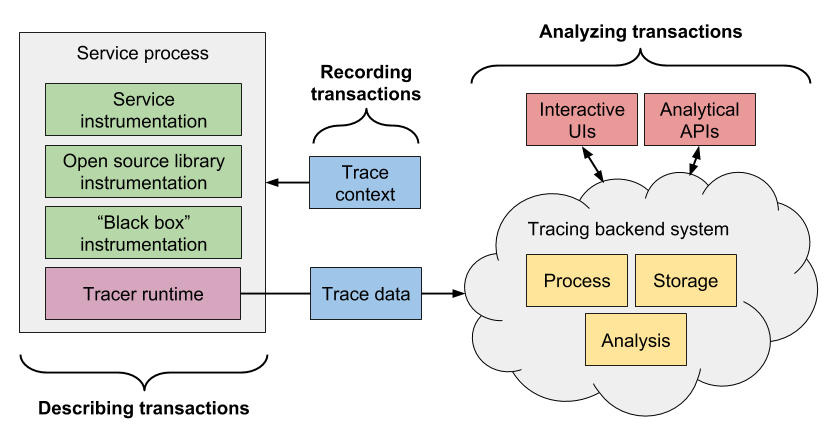
\includegraphics[scale=0.5]{pictures/tracing_concept.png}
		\end{center}
		\legend{Fonte: \url{https://cdn-images-1.medium.com/max/838/1*NuwuCvqZHLBJcJycRr1HTw.png}}
	\end{figure}
	
	\begin{figure}[htb]
		\caption{\label{fig_tracing_components}Componentes de um Distributed Tracing}
		\begin{center}
		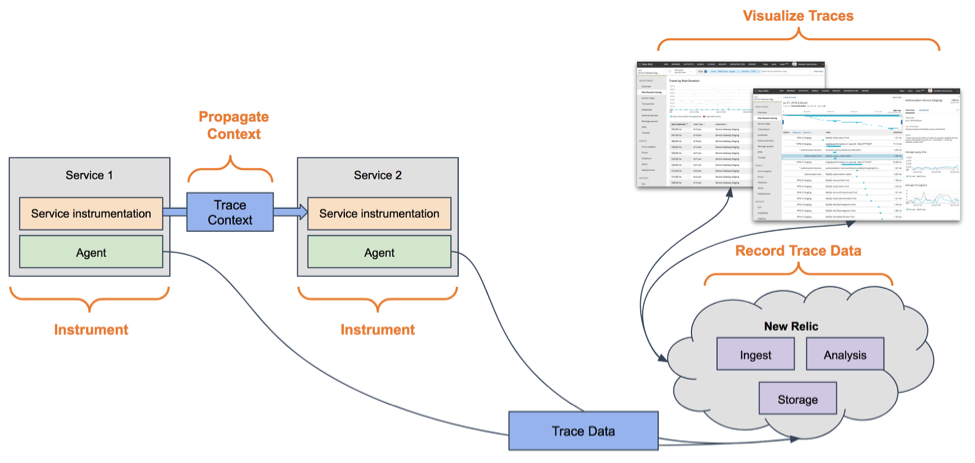
\includegraphics[scale=0.95]{pictures/distributed-tracing-components.png}
		\end{center}
		\legend{Fonte: \url{http://blog.newrelic.com/wp-content/uploads/Distributed-tracing-components.png}}
	\end{figure}
	
	Um dos primeiros Distributed Tracers que foi desenvolvido, foi o Dapper \cite{googledapper}, pela Google em meados de 2010. Com a abertura do código do Dapper outras empresas acabaram se interessando pelo projeto e funcionalidades e criaram suas próprias versões de tracers, entre eles alguns dos mais famosos: Zipkin\cite{zipkin}, pelo Twitter, e Jaeger\cite{jaegerarch}, pela Uber. Com o surgimento de novos tracers no mercado, a industria entrou em busca de um padrão para esse tipo de software, originando-se o OpenTracing\cite{opentracing}. OpenTracing é um padrão desenvolvido afim de definir normas e regras e padrões para implementação de Distributed Tracers. Nela são descritos estratégias para se realizar a identificação de informações gera mente importantes e o formato do tráfego de dados entre os serviços e os brokers.
	
	Grande parte do valor dos Distributed Tracing vem de suas ferramentas analíticas, que facilitam a vida do desenvolvedor e permitem com que ele faça análises de forma rápida e eficiente nos sistemas. Geralmente essas ferramentes vem junto com uma aplicação de Frontend que consegue exibir fluxos e montar gráficos. Entre eles o Flamegraph é muito utilizado para visualizarmos como a comunicação se aprofunda e se propaga na rede, uum exemplo de Flamegraph do Zipkin pode ser visto na figura \ref{fig_zipking_sample}. Outro tipo de visualização muito útil é a de mapa de Topologia de servços, que nada mais é que um grafo representando as interações entre diversos serviços, temos um exemplo na figura \ref{fig_topology_map}
	
	\begin{figure}[htb]
		\caption{\label{fig_zipking_sample}Exemplo de Flamegraph do Zipkin}
		\begin{center}
		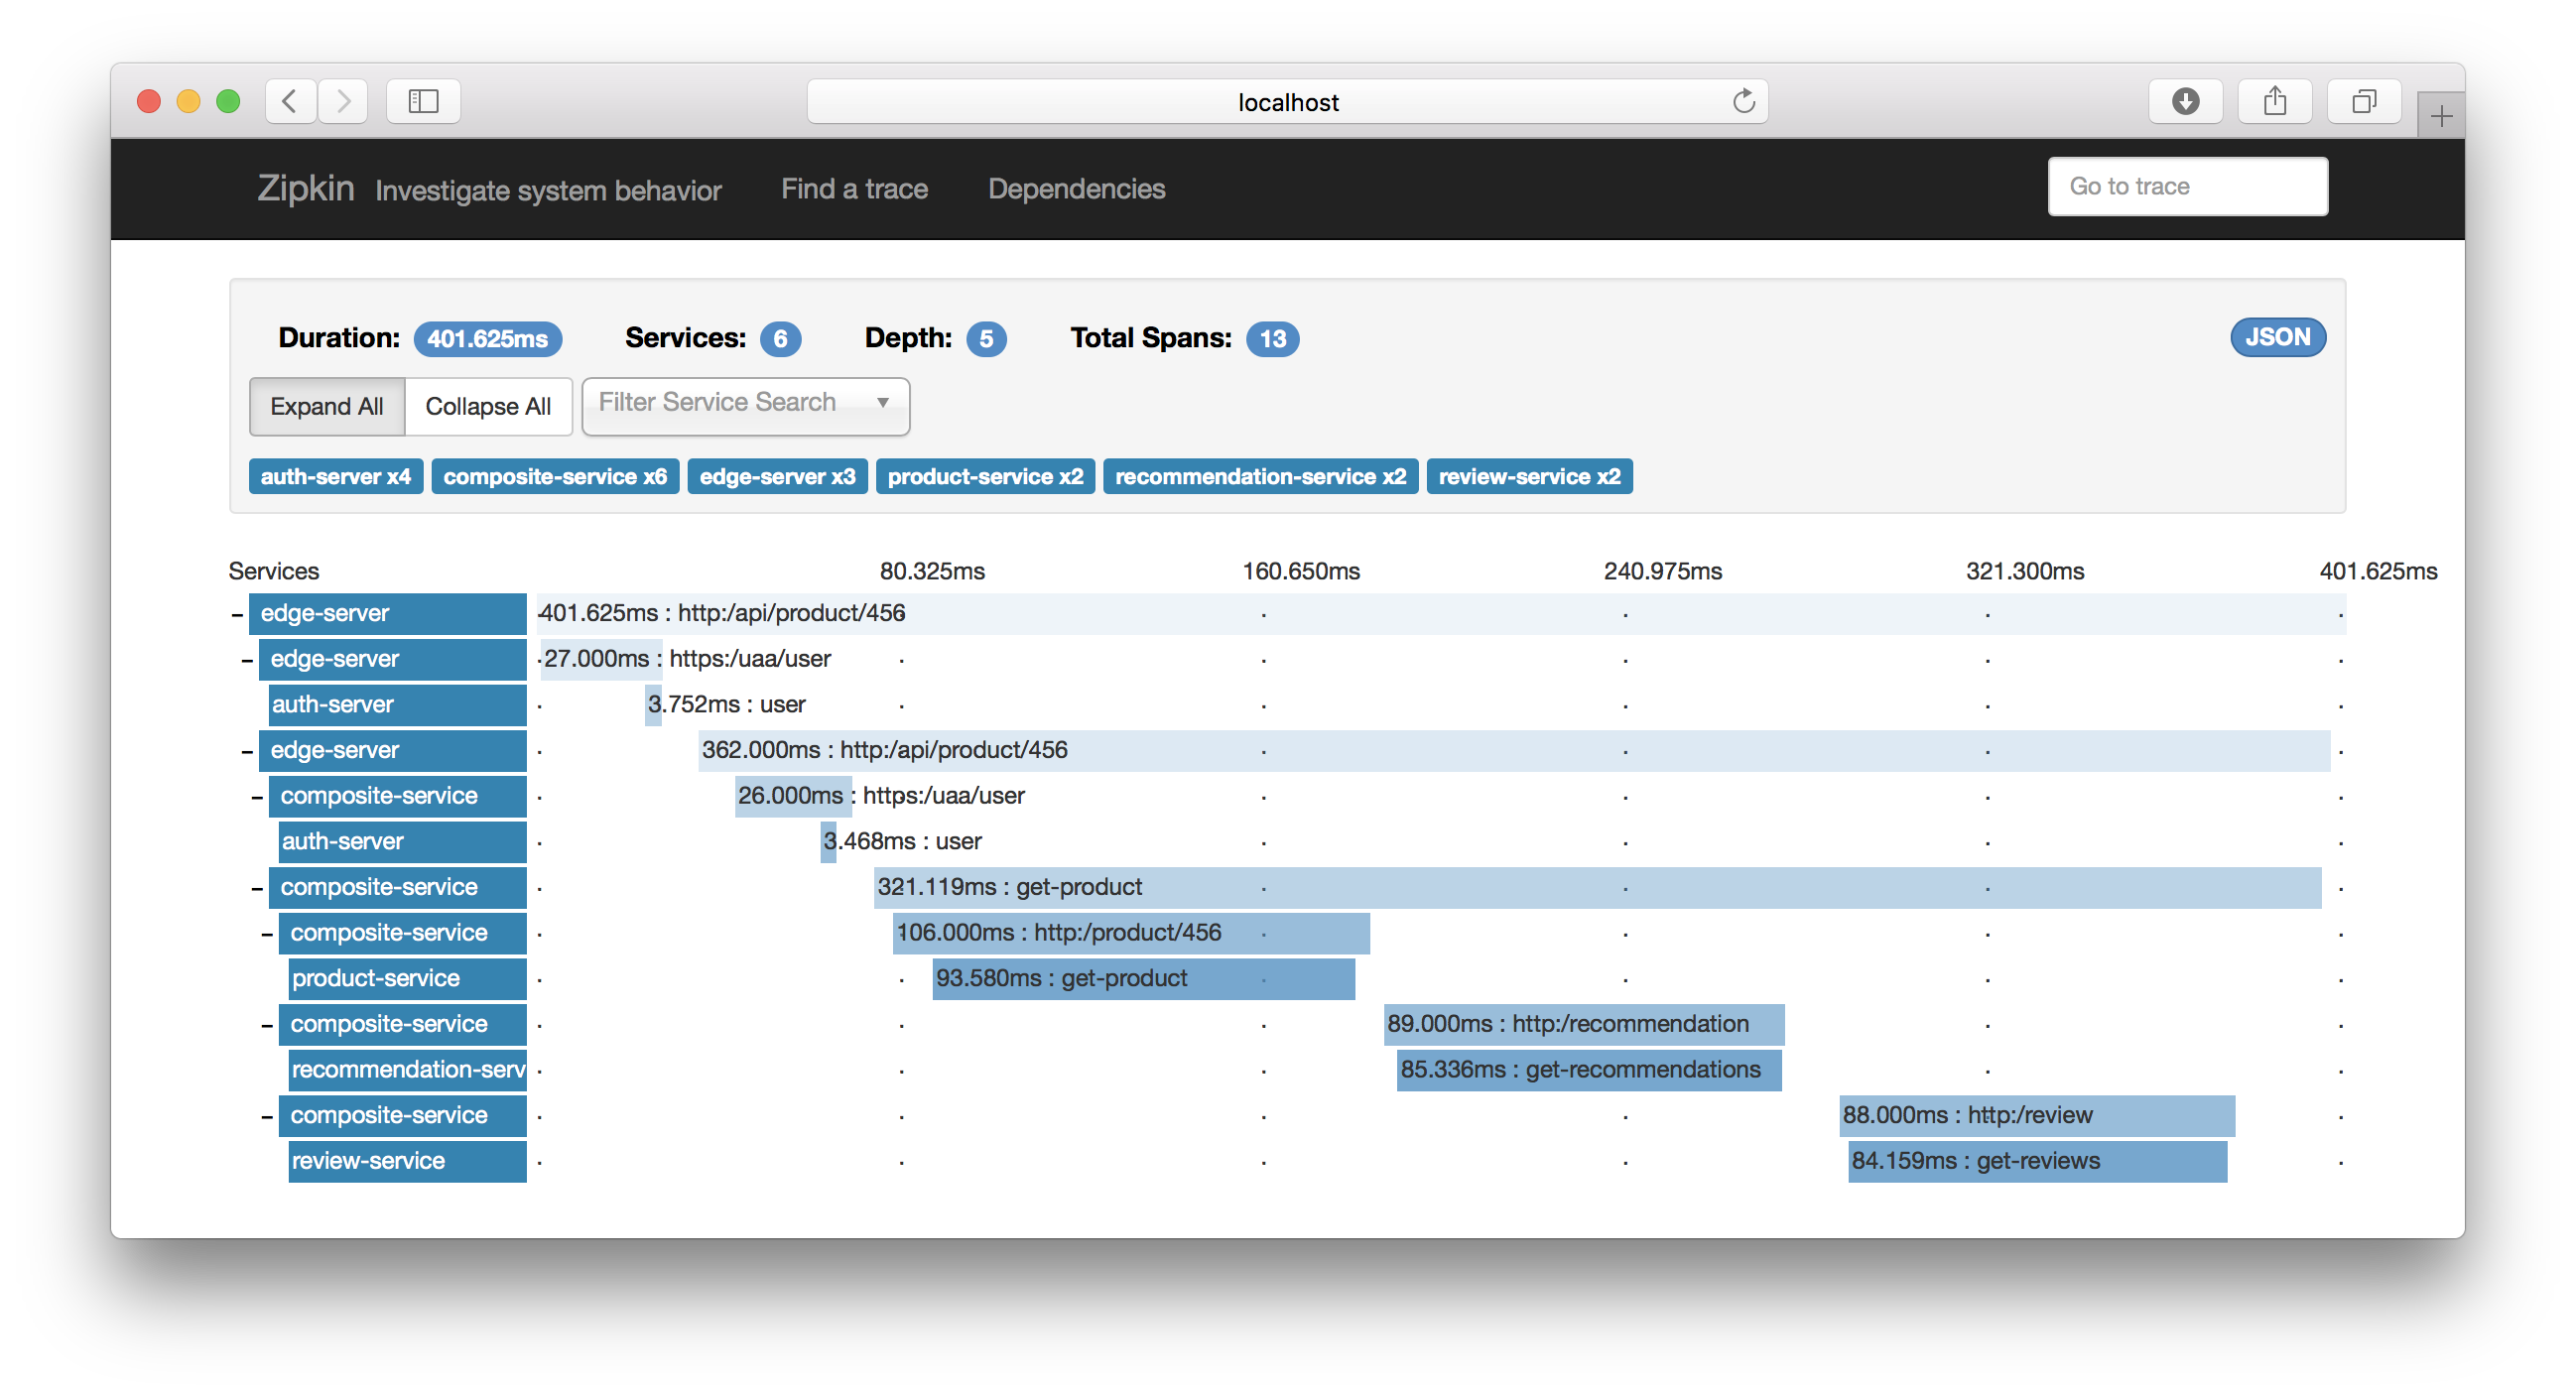
\includegraphics[scale=0.16]{pictures/zipkin-sample.png}
		\end{center}
		\legend{Fonte: \url{http://callistaenterprise.se/assets/blogg/build-microservices-part-7/Zipkin-sample.png}}
	\end{figure}
	
	\begin{figure}[htb]
		\caption{\label{fig_topology_map}Exemplo de Mapa de Topologia de Serviços}
		\begin{center}
		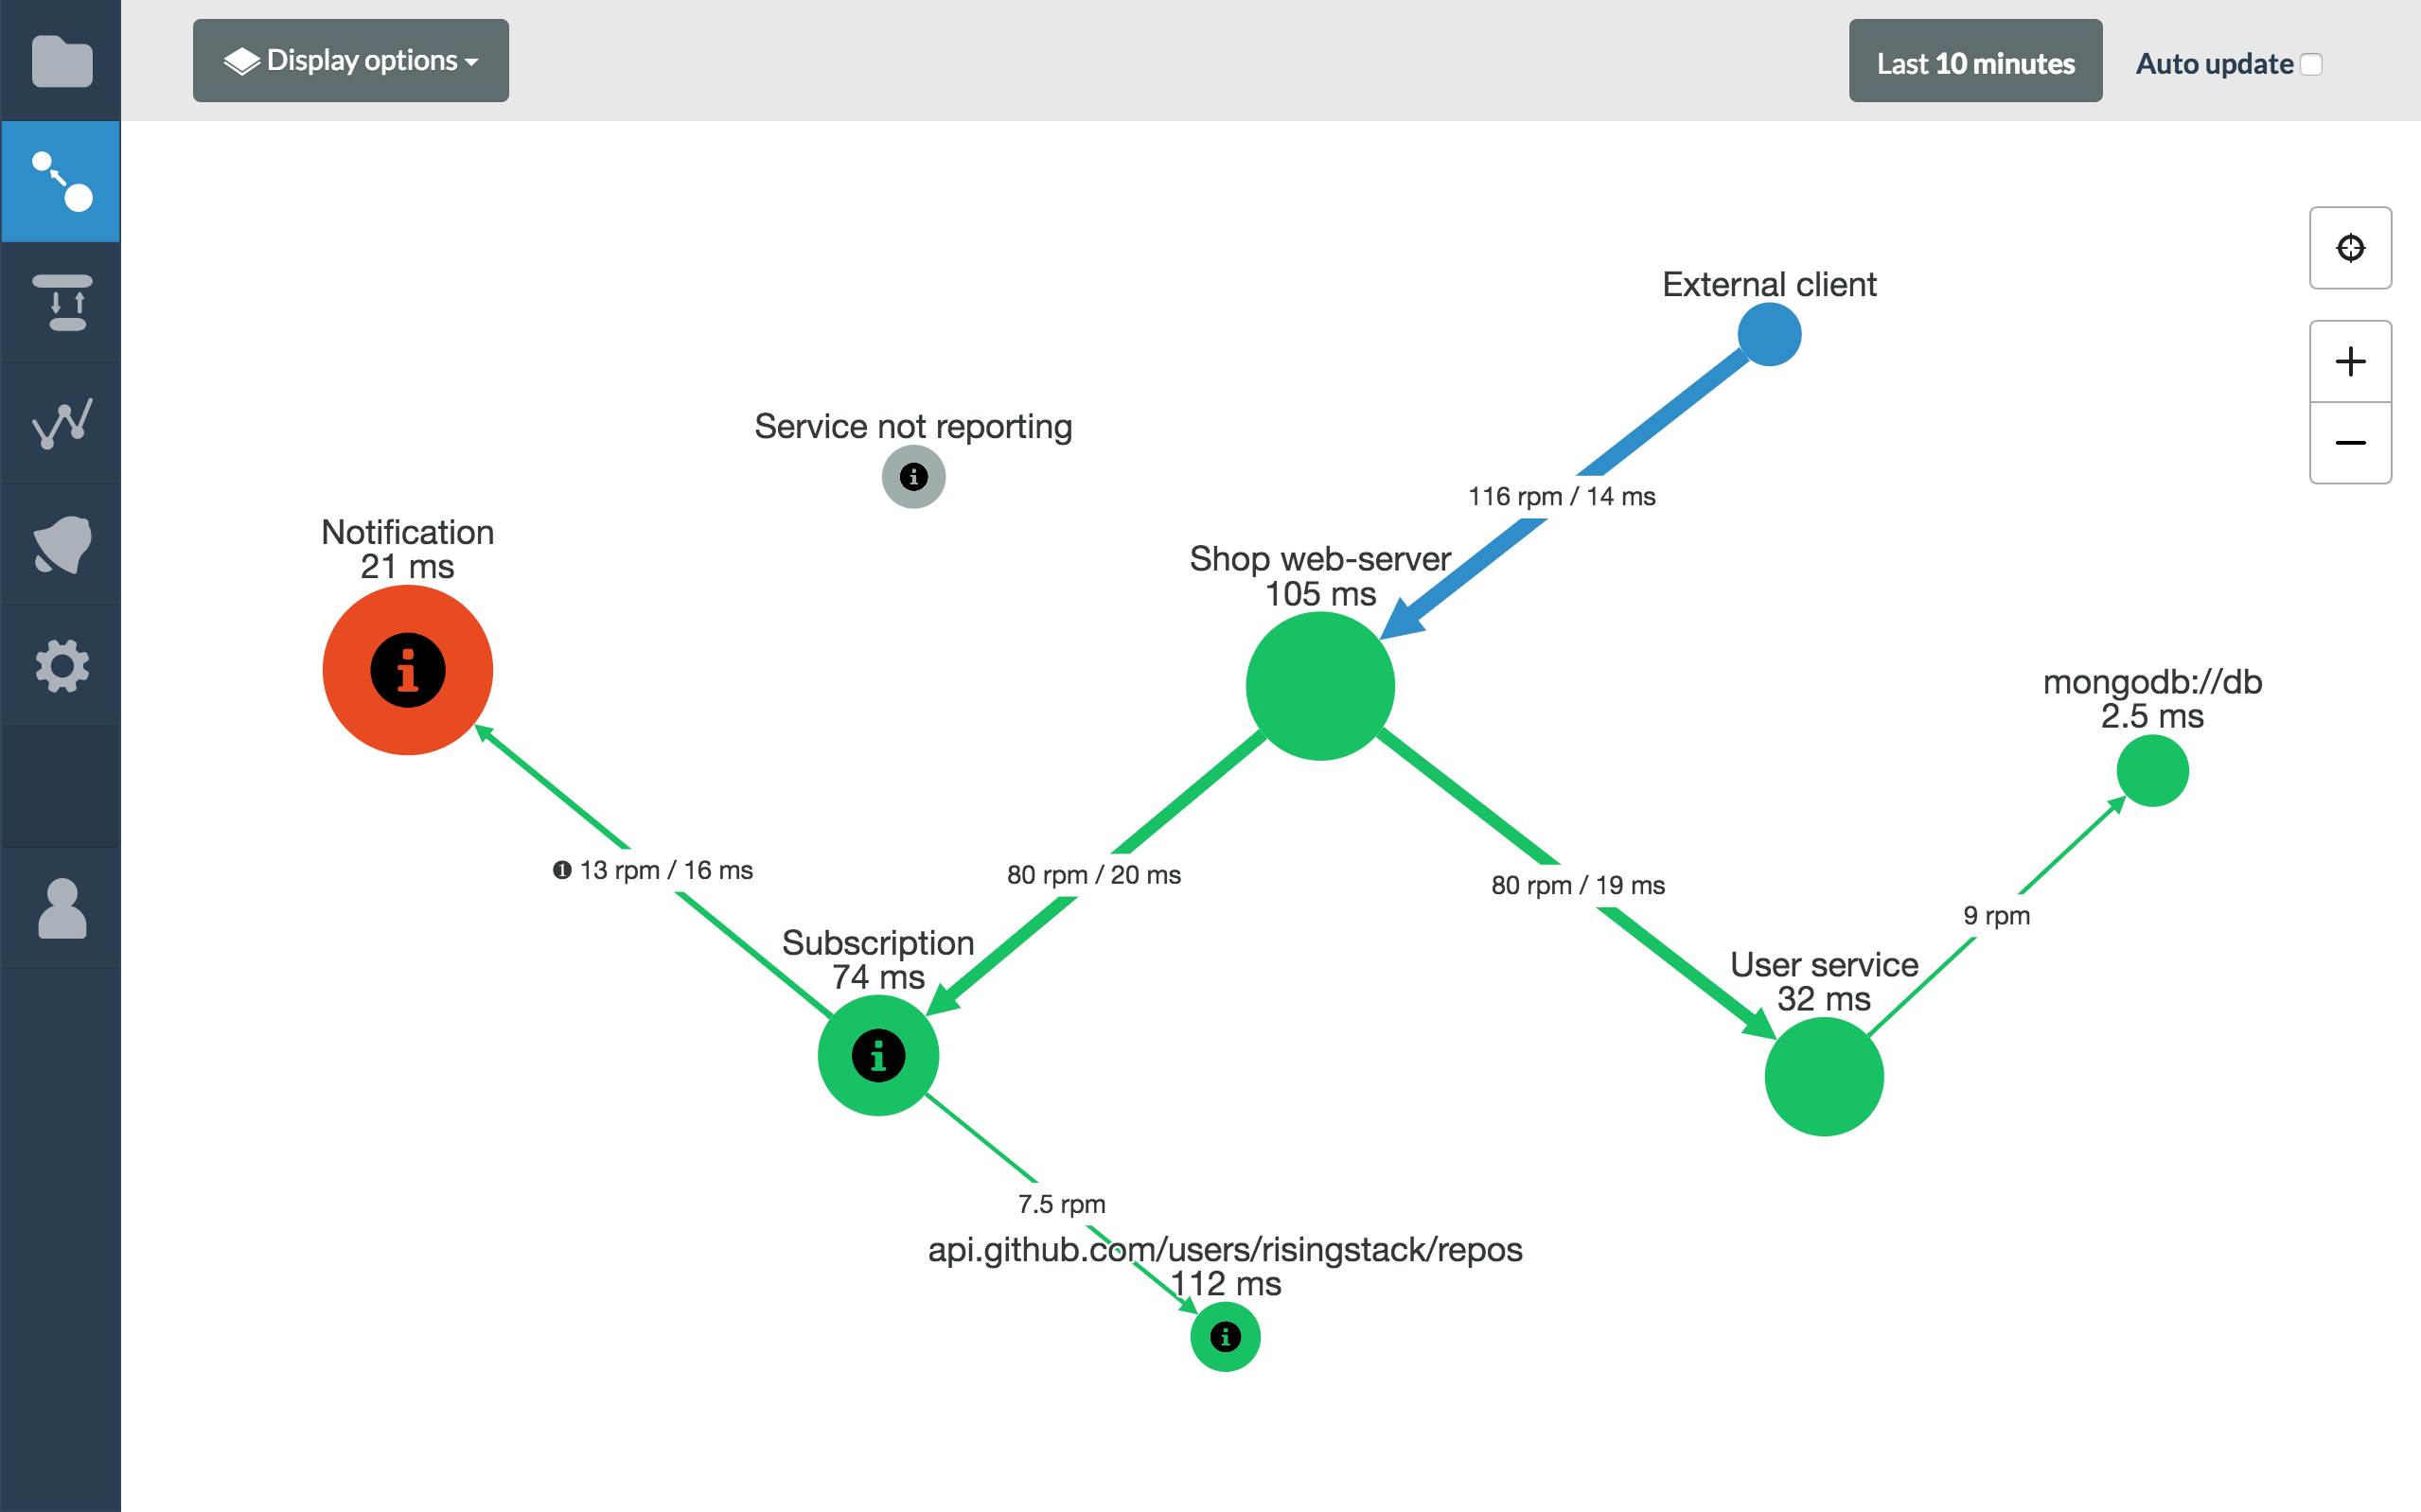
\includegraphics[scale=0.16]{pictures/service_topology_map.png}
		\end{center}
		\legend{Fonte: \url{https://blog-assets.risingstack.com/2016/May/Distributed_transaction_tracing_with_service_topology_map_trace_by_risingstack-1462456507669.png}}
	\end{figure}
	
	\section{Devspaces}
    
    Um Devspace, como foi batizado pelo grupo, é um ambiente de desenvolvimento isolado que roda em cima da plataforma Formicarium. Ele é o ambiente que o desenvolvedor vai ter disponível para uso e que vai interagir durante o seu tempo testando e desenvolvendo os serviços. 
    
    Os Devspaces são provisionados e configurados de forma automática pelo serviço Soil, a medida que um desenvolvedor requisita sua criação através da CLI. Para obter dados de configuração e setup inicial do Devspace, o Soil consulta um servidor de configurações via Webhooks, esse encarregado de fornecer todo configuração específica da empresa para fazer o bootstrap de um novo Devspace.
    
    Objetivamente, os Devspaces são Namespaces do Kubernetes que são gerenciados pelo Soil, além dos recursos padrões do Kubernetes, esse Namespaces acabam recebendo serviços adicionais do Formicarium, sendo esses o Hive e o Tanajura. A interação com os Devspaces é feito sempre através da CLI do Formicarium, não exigindo que o usuário tenha que ter o ferramental do Kubernetes instalado e configurado em sua máquina.
    
    Dentro de um Devspace os serviços que rodam nele conseguem se localizar entre si por meio do servidor de DNS do Kubernetes que garante isolamento entre Namespaces, dessa forma conseguimos alcançar um isolamento entre serviços entre Devspaces, mesmo que 2 desenvolvedores estejam executando o mesmo serviço. Além disso, cada Devspace recebe do Config Server um conjunto de aplicações de infra-estrutura ou de uso comum, que também garante isolamento dos demais Devspaces, como por exemplo, a existência de um broker de mensageria por Devspace. não havendo confusão na produção e consumo de mensagens.
    
        \begin{figure}[htbp]
			\caption{\label{fig_devspace1}Anatomia de um Devspace}
			\begin{center}
			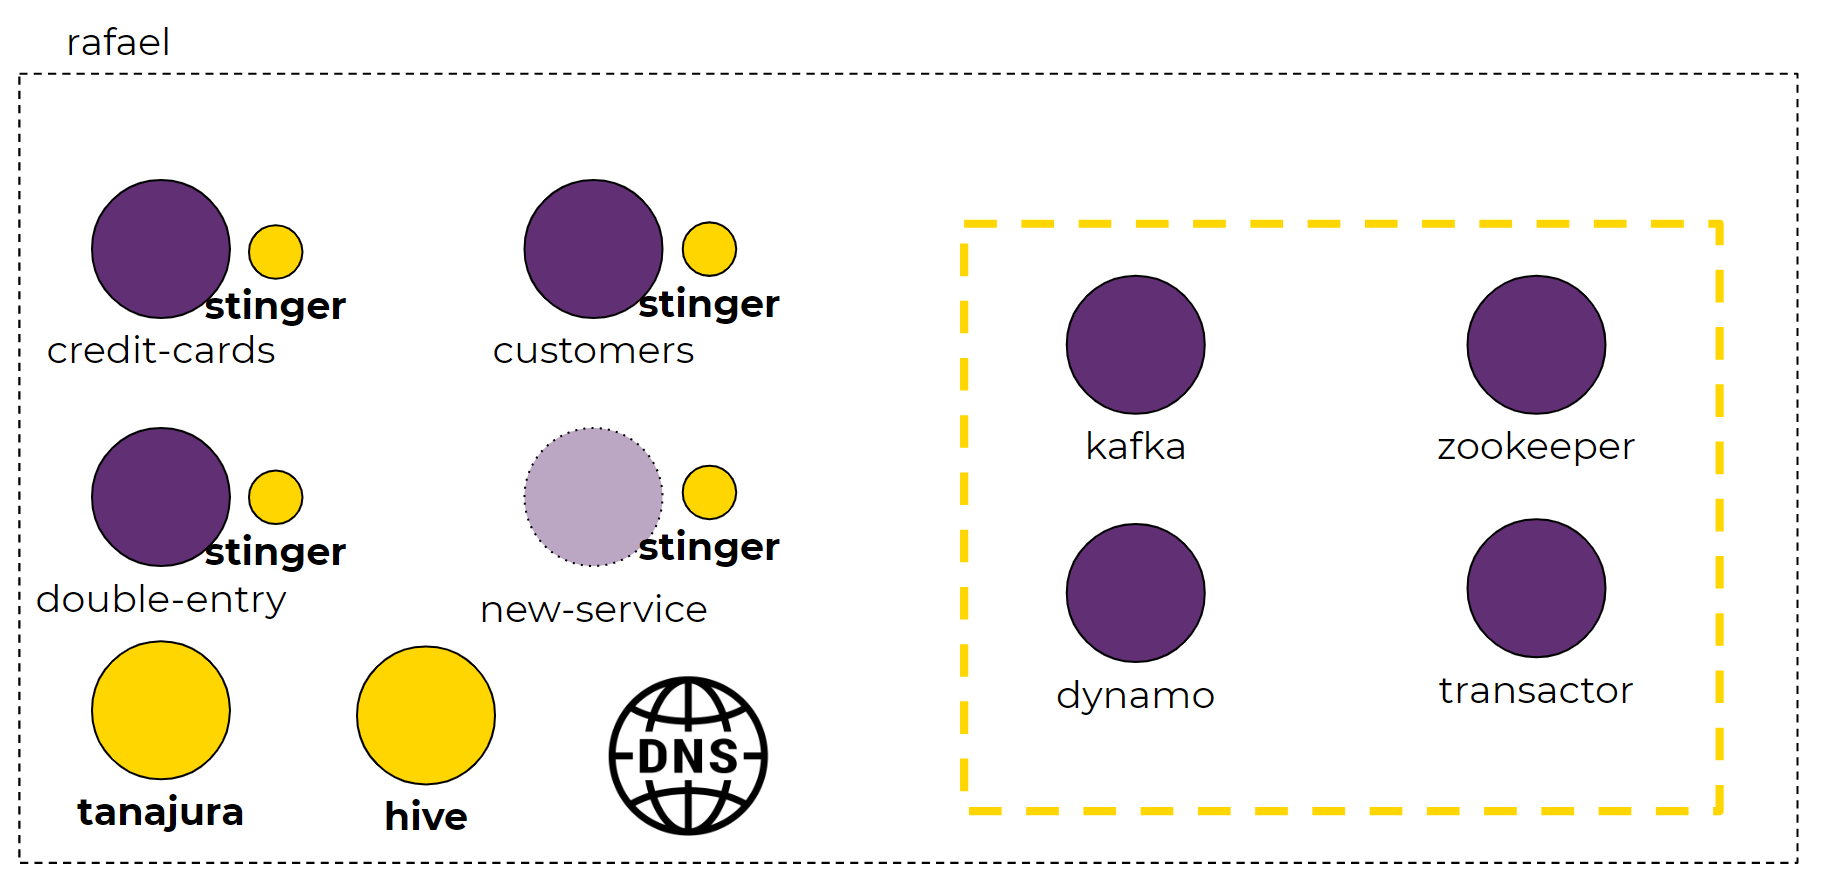
\includegraphics[scale=0.30]{pictures/devspace1.png}
			\end{center}
			\legend{Fonte: os autores}
			% \caption{Fonte: própria}
		\end{figure}
    
    	\begin{figure}[htbp]
			\caption{\label{fig_create_devspace}Fluxo de Criação de Devspaces}
			\begin{center}
			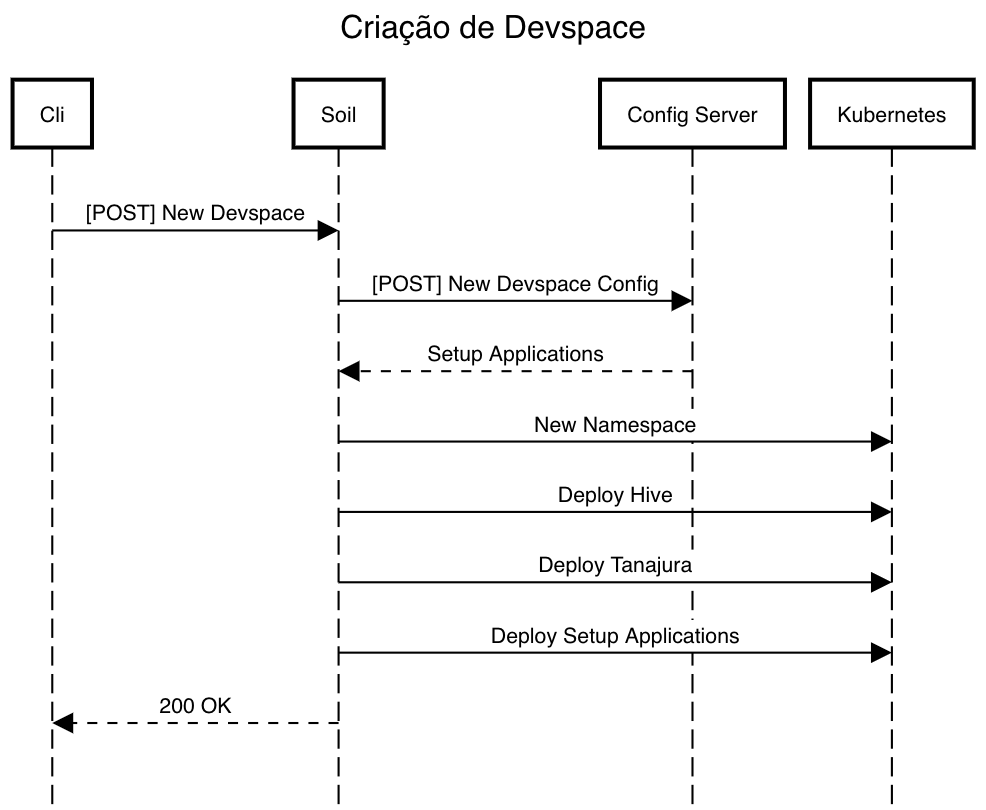
\includegraphics[scale=0.40]{pictures/create-devspace.png}
			\end{center}
			\legend{Fonte: os autores}
			% \caption{Fonte: própria}
		\end{figure}